\documentclass[12pt,journal,compsoc]{IEEEtran}

\usepackage[english]{babel}
\usepackage[utf8]{inputenc}
\usepackage[cmex10]{amsmath}
\usepackage{graphicx}
\usepackage[colorinlistoftodos]{todonotes}
\usepackage{tikz}
\usepackage{subfigure}
\usetikzlibrary{shapes, shadows, arrows}
\usepackage{float}
\usepackage{color}
\usepackage{hyperref}
\usepackage{fancyhdr}
\pagestyle{fancyplain}

\begin{document}

\title{\Huge Breast Cancer Prediction \& Classification Using Machine Learning }

\author{Shah Rutvik Vrajesh
\\ NITC CSE M180324CS
}

\maketitle

\IEEEdisplaynontitleabstractindextext

\IEEEpeerreviewmaketitle


\IEEEtitleabstractindextext{
\begin{abstract} 
  Cancer is a class of diseases, which is driven by
change in cells of the body and increase beyond normal
growth and control. Breast cancer is one of the frequent types
of cancer.
   In today’s world Breast cancer is one of the main
problems faced by women. Identifying cancer is the first stage and
is always challenging. 
    Detection and nursing of the breast cancer
have become an urgent. Early treatments of breast cancer have become an
extremely crucial work to do, not only helps to cure cancer but
also helps in curative of its incidence.
        With the advancement of technology and
machine learning techniques, the cancer diagnosis and
detection accuracy has improved.
        Today, there are different
kinds of methods and Machine Learning techniques and diverse process
like knowledge discovery are developed for anticipating breast
cancer.
Machine learning (ML)
techniques offer various probabilistic and statistical methods
that allow intelligent systems to learn from reoccurring past
experiences to detect and identify patterns from a dataset.
The aim of this research
work is to predict breast cancer, which is the second leading
cause of death among women worldwide, and with early detection
and prevention can dramatically reduce the risk of death, using
several machine-learning algorithms.
The research work presented an overview of evolve the
machine learning techniques in cancer disease by applying
learning algorithms on breast cancer dataset like–Linear
regression, Random Forest, Multi-layer Perceptron , Naive Bayes (NB)
classifier and knearest neighbor (KNN),SVM,
Decision Trees (DT),etc. The result outcome shows that
which one performs better than other techniques.

%As per the survey, I perform a comparison of various learning techniques
%on same dataset.



  



\end{abstract}

\begin{IEEEkeywords}
    Machine Learning, Classification,Prediction, Breast cancer,
\end{IEEEkeywords}}

\section{Abstract}

\IEEEPARstart{C}{a} 
  ncer is a class of diseases, which is driven by
change in cells of the body and increase beyond normal
growth and control. Breast cancer is one of the frequent types
of cancer.
   In today’s world Breast cancer is one of the main
problems faced by women. Identifying cancer is the first stage and
is always challenging. 
    Detection and nursing of the breast cancer
have become an urgent. Early treatments of breast cancer have become an
extremely crucial work to do, not only helps to cure cancer but
also helps in curative of its incidence.
        With the advancement of technology and
machine learning techniques, the cancer diagnosis and
detection accuracy has improved.
        Today, there are different
kinds of methods and Machine Learning techniques and diverse process
like knowledge discovery are developed for anticipating breast
cancer.
Machine learning (ML)
techniques offer various probabilistic and statistical methods
that allow intelligent systems to learn from reoccurring past
experiences to detect and identify patterns from a dataset.
The aim of this research
work is to predict breast cancer, which is the second leading
cause of death among women worldwide, and with early detection
and prevention can dramatically reduce the risk of death, using
several machine-learning algorithms.
The research work presented an overview of evolve the
machine learning techniques in cancer disease by applying
learning algorithms on breast cancer dataset like–Linear
regression,Artificial Neural Netork, Random Forest, Multi-layer Perceptron , Naive Bayes (NB)
classifier and knearest neighbor (KNN),SVM,
Decision Trees (DT),etc. The result outcome shows that
which one performs better than other techniques.

%%\begin{flushright}
    %%{\textit{Hay una fuerza motriz\\
    %%más poderosa que el vapor,\\
    %%la electricidad y la\\
    %%energía atómica: la voluntad.}\\
%%\textbf{Albert Einstein (1879-1955).}}
%%\end{flushright} 

%%\section{Desarrollo de la Práctica}

%%Para el desarrollo de la práctica, los estudiantes deberan contar con los siguientes materiales:\\

%%\begin{itemize}
%%\item Protoboard.
%%\item Resistencias de varios valores.
%%\item Potenciómetro.
%%\item Batería de 9V.
%%\item Porta-batería.
%%\item Cable de conexión para protoboard.
%%\item Pelaclables, pinza, cortafrío.\\
%%\end{itemize}

%%Además de los anteriores elementos, los estudiantes 
%%\subsection{Conocimiento del laboratorio}
%%Antes de iniciar la práctica, se realizará una normas de seguridad requeridas.\\

%%Posteriormente, uno de los estudiantes del grupo de trabajo se desplazará para realizar el préstamo de los elementos y la estación de trabajo requerida.

%%\subsubsection{Desarrollo de la Práctica}
%%Para el desarrollo de la práctica, los integrantes del grupo deberán implementar un circuito serie como el presentado en la figura \ref{fig1}. Este circuito debe estar simulado antes de iniciar la práctica para tener el conocimiento previo de los resultados que se quieren obtener.\\

%%\begin{figure}[!ht]
%%\centering
%%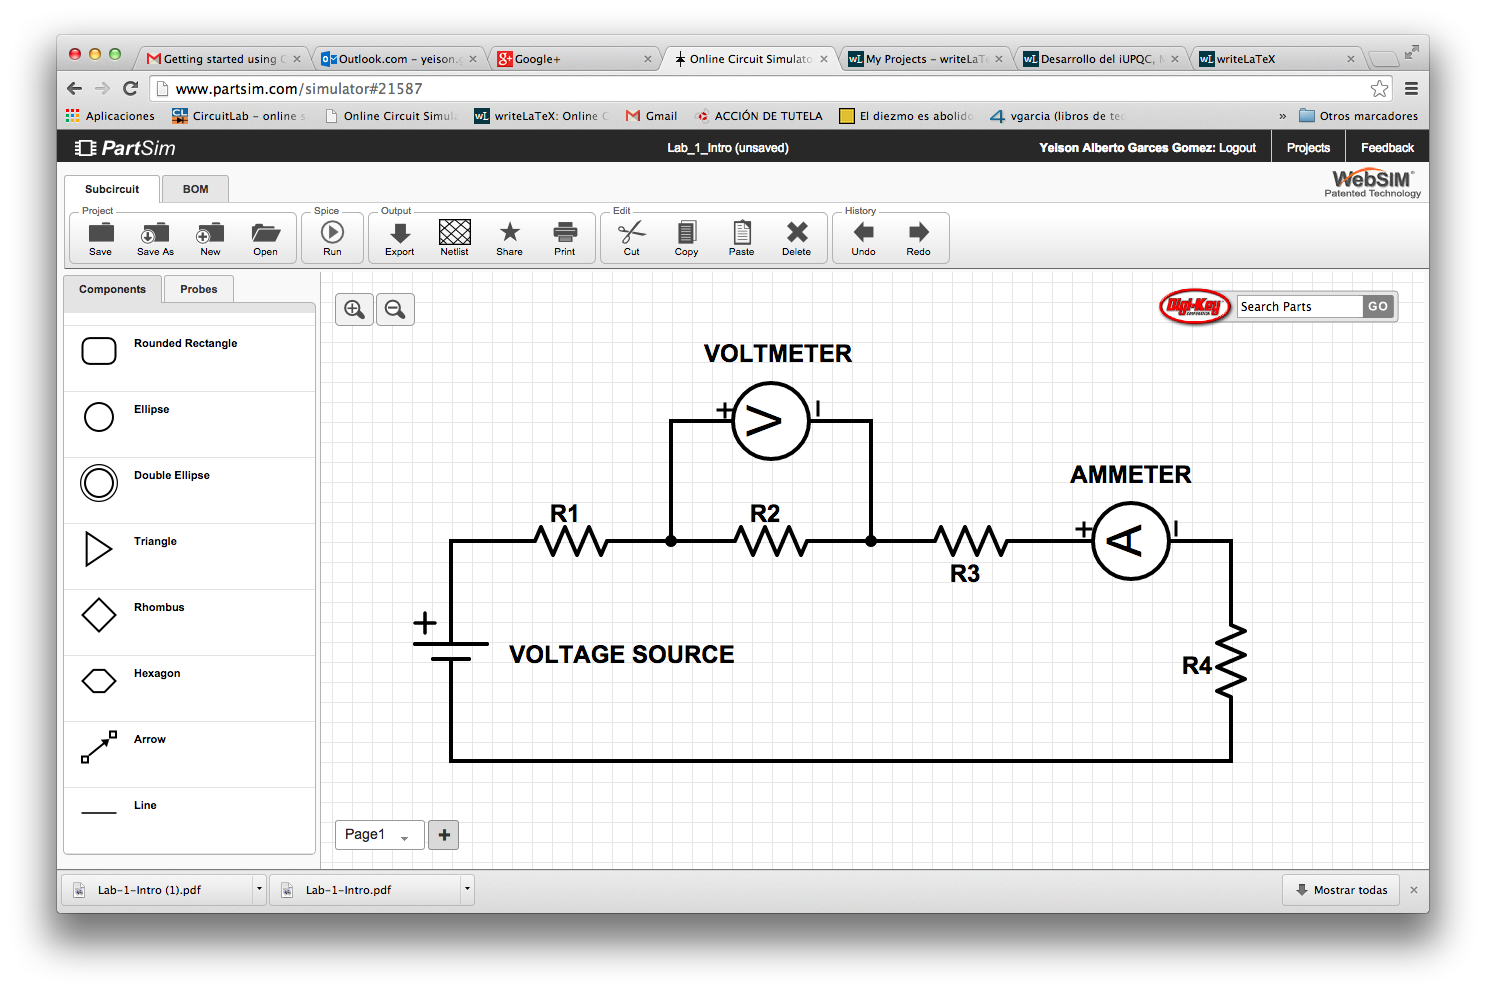
\includegraphics[trim = 0.0cm 0.0cm 0.0cm 0.0cm, clip, width=0.48\textwidth]{fig1.png}
%%\caption{\label{fig1}Circuito serie.}
%%\end{figure}

%%Los valores de las resistencias deberán estar de acuerdo a los mismos valores simulados.\\

%%\section{Sustentación e Informe}
%%La nota de cada práctica se compone de lo siguiente:\\

%%\begin{enumerate}
%%\item El montaje del circuito y su correcto funcionamiento, para este caso es necesario que los estudiantes en lo posible lleguen con el circuito ya montado en su protoboard correspondiente y que las conexiones estén ordenadas, en ningún caso se aceptará montajes con cables por encima de los elementos o que no sea posible hacerles un seguimiento. Por favor referirse a la figura \ref{orden} para entender el montaje que se aceptará en la práctica.
%%\item Una sustentación por cada uno de los estudiantes del grupo.
%%\item La presentación de las simulaciones
%%\item Un informe de la práctica en \LaTeX, éste debe contener:
%%\begin{itemize}
%%\item introducción
%%\item desarrollo de la práctica
%%\item simulación
%%\item discusión de resultados
%%\item conclusiones
%%\end{itemize}
%%\end{enumerate}

%%\begin{figure}[h!]
%% \centering
%% \subfigure[Circuito desordenado]{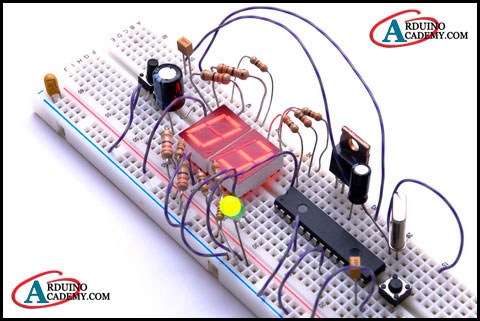
\includegraphics[width=0.3\textwidth]{proto1.jpg}}
%% \subfigure[Circuito ordenado]{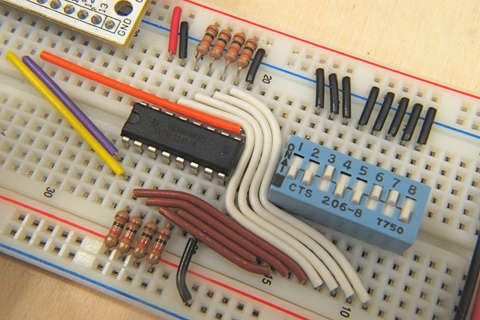
\includegraphics[width=0.3\textwidth]{proto2.jpg}}
%% \caption{demostración de como deben estar implementados los circuitos}
%% \label{orden}
%%\end{figure}

%%\ifCLASSOPTIONcompsoc
%%  \section*{Acknowledgments}
%%\else
%%  \section*{Acknowledgment}
%%\fi

%%Los autores agradecen a overleaf.com y a partsim.com.

%%\ifCLASSOPTIONcaptionsoff
 %% \newpage
%%\fi


\begin{thebibliography}{1}
\bibitem{}Alireza Osareh , Bita Shadgar ,"Machine Learning Techniques to Diagnose Breast
Cancer"
\\
\bibitem{}Siyabend Turgut , Mustafa Da÷tekin and Tolga Ensari ,"Microarray Breast Cancer Data Classification Using
Machine Learning Methods"
\\
\bibitem{}Zahra Nematzadeh, Roliana Ibrahim, Ali Selamat , "Comparative Studies on Breast Cancer
Classifications with K-Fold Cross Validations Using
Machine Learning Techniques"
\\
\bibitem{}D.Pavithra , Mr.B.Lakshmanan ,"Feature Selection and Classification in gene
expression cancer data"
\\
\bibitem{}GOPAL K. DHONDALAY, DONG L. TONG, GRAHAM R. BALL ,ESTROGEN RECEPTOR STATUS PREDICTION FOR BREAST CANCER
USING ARTIFICIAL NEURAL NETWORK""
\end{thebibliography}

\end{document}